% ==================================================
%
%   模型的建立与求解
%
% --------------------------------------------------

\section{模型的建立与求解}

\begin{figure}[h]
    \centering
    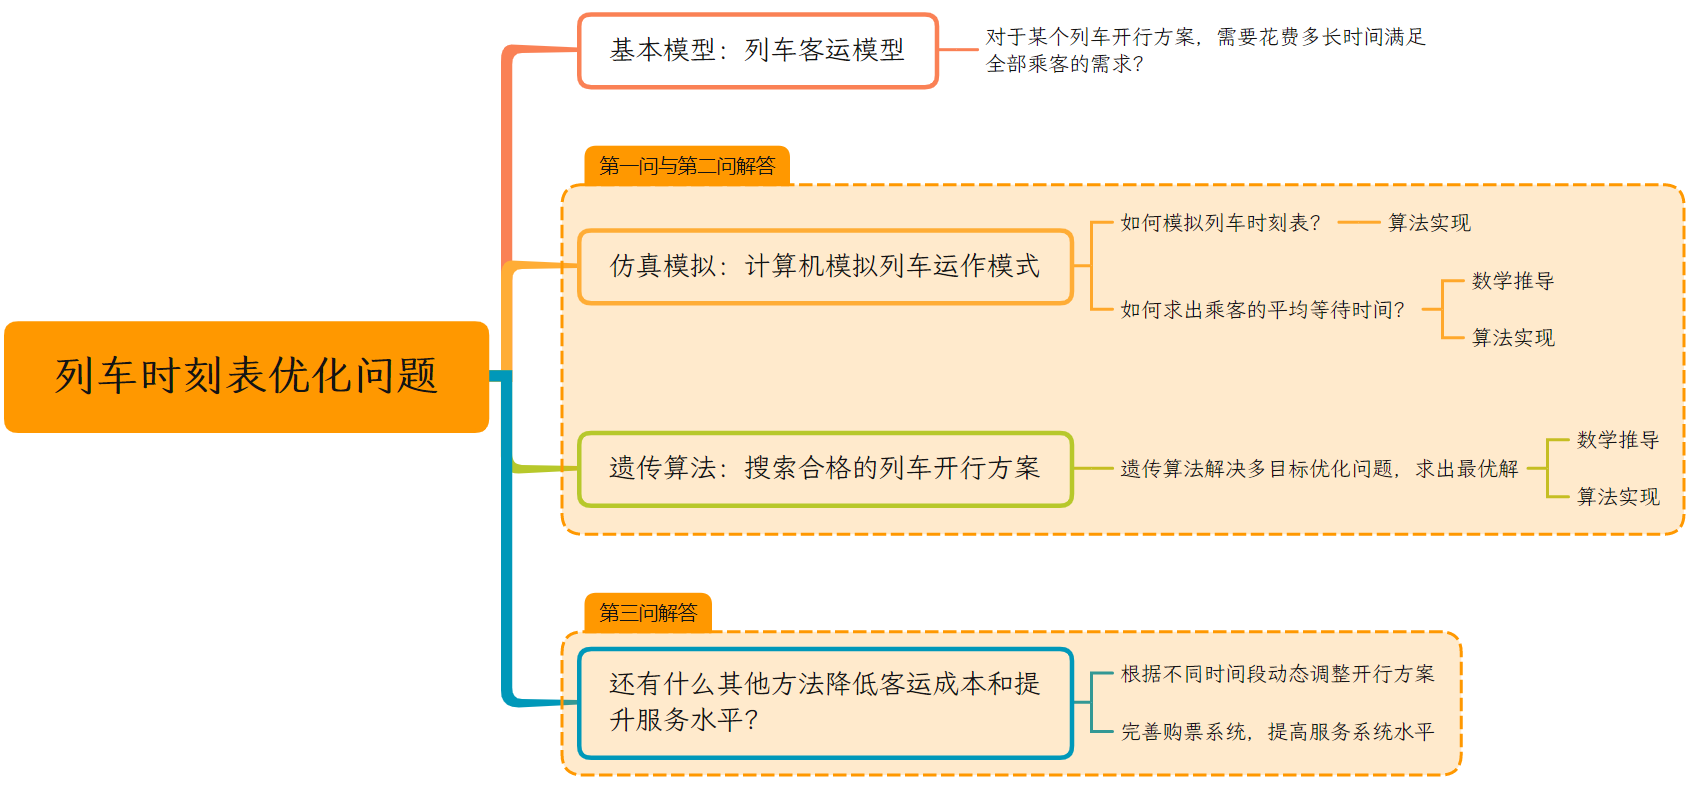
\includegraphics[scale=0.2]{res/figure161100.png}
    \caption{模型思维图}
\end{figure}

% ............ 模型的准备 ............ %

\subsection{模型的准备}

为了方便后续对问题的分析和建立,这里先给出\textbf{列车客运模型}与\textbf{遗传算法}的概述,旨在方便读者更好的理解解题模型的核心思想。

\subsubsection{列车客运模型}

列车客运模型是一种简化的列车运行模型。

为了方便表述,考虑只有$5$个车站的情况。在这$5$个车站中,从前到后依次标号为$1-5$。设发车的间隔时间为$\Delta t$,那么在该开行方案下,需要耗费多长时间才能满足所有乘客的需求?

利用列车行程图,可以清晰的展现出列车的运行模式。

\begin{figure}[h]
    \centering
    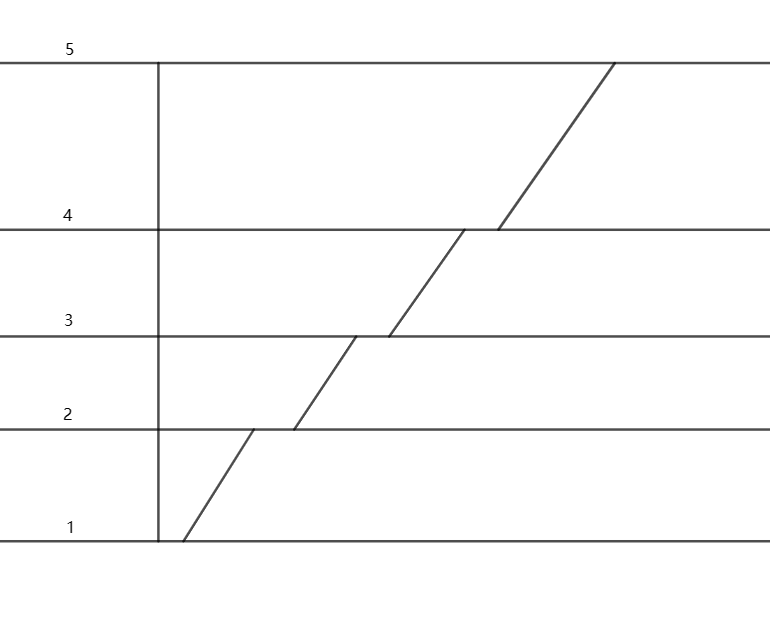
\includegraphics[scale=0.3]{res/figure160314.png}
    \caption{列车运行图}
\end{figure}

考虑现实情况以及OD客流数据,每趟列车上车的乘客是按照乘客需求的比例分配的。例如,在车站$1$时,某一次的上车乘客比例于OD客流数据比例相等。但是伴随着后面的列车的运行过程,因为下车的乘客数量是不一定的所以说,下车的时间是不一定的。为了考虑这样的情况,我们必须要给出很多合理的解释。这是因为原本在这个车站下车的人数就有所变化,对于这种非数值计算类问题,在文后将尝试采用程序模拟的办法的最后的运行结果,而求出我们最开始给出的问题——需要耗费多长时间才能满足所有乘客的需求?

该模型主要功能是描述列车的运行模式,为接下来的仿真模型做出准备。

\subsubsection{遗传算法简介}

遗传算法(Genetic Algorithm, GA)也被称为进化算法(Evolutionary Algorithm)。该算法是一种仿生算法,旨在通过模仿生物遗传演化机制,达到优化群落的目的\cite{hanJiyuyichuanheshengsuanfaqiujiehanshuyouhuawenti2010}。为了更好的理解遗传算法,让我们回顾一下自然界中生物的演化是如何进行的?

生物学表明,生物的演化是以种群为单位的,而演化的本质是基因的变异。

还有个更重要的东西——自然选择。或者通俗的理解为,种群对环境的适应度。宏观上看的话,种群是朝着适应度高的方向进行的。

根据以上论述,可以提炼出遗传算法的三个要素:

\begin{enumerate}
    \item 种群——基因与染色体
    \item 演化
    \item 适应度
\end{enumerate}

在遗传算法中,首先可以根据随机数算法生成初始群落。紧接着使该种群中的个体相互交配繁衍,产生新的个体。在产生新的个体的过程中,要确保完成两个操作:染色体的交叉互换和基因变异。前者保证优秀的基因有可能配对在一起,后者保证了种群的基因多样性,防止种群的基因趋同,这样可以防止算法陷入局部最优解。产生了下一代以后,接下来计算出所有个体的适应度,剔除适应度最低的那几些个体,使得产生个体数量与初始群落一致的第二代群落。最后一次遗传算法的迭代就已经完成(如图\ref{GeneticAlgorithmDiagram})。

设定遗传算法迭代的终止,最后得到的种群就是最优解集,可以取最高适应度作为最终的解。

\begin{figure}[h]
    \centering
    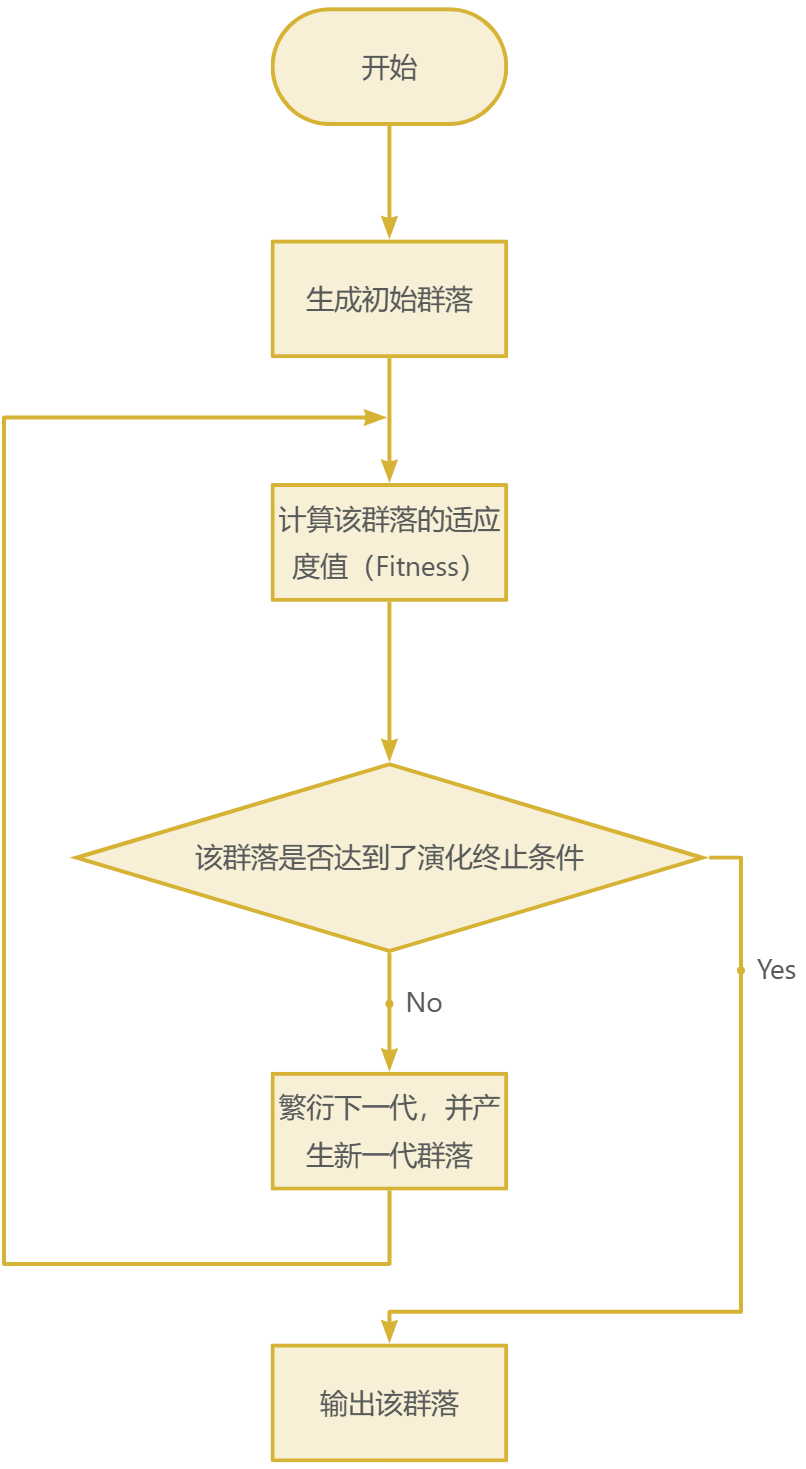
\includegraphics[scale=0.15]{res/GeneticAlgorithmDiagram.png}
    \caption{遗传算法框图}
    \label{GeneticAlgorithmDiagram}
\end{figure}

实际上,遗传算法最大的难点在于演化这一步骤。在一般算法中,演化有两个重要操作需要进行——基因互换和染色体的变异,可以说,对这两个操作的设计涵盖了整个遗传算法的绝大部分设计。


% ............ 模型的准备 ............ %

\subsection{问题$1$模型的建立与求解}

\subsubsection{仿真模拟计算:计算机模拟列车的运作模式}

为了求出相关的计算方法

\subsubsection{求出乘客的平均等待时间}

在站台$i$,乘客去$j$站台的频率为:希望从$i$站台到$j$站台的乘客人数,与该站台总乘客人数之比。

\begin{equation}
\alpha(i, j) = 
	\frac {M_f(i, j)}{\sum _{k = i} ^{30} M_f(i, k)}
\end{equation}

第$t$辆出发的列车“刚刚”到达$i$站时,车厢内正有$M_{cur}(i, j, t)$个乘客打算到$j$站。当该车站为起点站时,视为列车“刚到”起点站,也就是乘客还未上下车,因此初始人数为$0$,无论大交还是小交都是这样(大交站台$1$为起点,小交站台$s$为起点);当该车站不是起点时,刚到该车站时车厢内的乘客可以通过:刚到上一个站台时的车厢状态、上一个站台的下车乘客与上一个站台的上车乘客反映出来。

\begin{equation}
M_{cur}(i, j, t) = 
	\begin{cases}
	M_{cur}(i - 1, j, k) - M_{out}(i - 1, t) + M_{in}(i - 1, j, t)  & \text{ if }\sigma \\
	0  & \text{ otherwise }
	\end{cases}
\end{equation}

其$¥\sigma$为条件区域:

\begin{equation}
    \sigma = 
        \begin{matrix}
 		1 < i \leq 30, (t - 1) < N_l \mod (N_l + N_s),  \\
		\text{ or } s < i \leq e, (t - 1) \geq N_l \mod (N_l + N_s)\\
		\end{matrix} \\
\end{equation}

第$t$辆发车的列车到第$i$个站台时,无论乘客的起点在哪,在该站台下车的乘客都会下车,即下车人数为:列车刚到这一站台时,所有目标在这一站台下车的本列车乘客总数,无论是乘坐大交还是乘坐小交都是这样。特别地,由于小交的范围不会超过大交的范围,因此:小交内在不在运行范围的车站的下车乘客人数视为$0$。

\begin{equation}
M_{out}(i, t) = 
	\begin{cases}
	\sum _{k = 1} ^{i} M_{cur}(k, i, t)  & \text{ if } (t - 1) < N_l \mod (N_l + N_s) \\
	\sum _{k = s} ^{i} M_{cur}(k, i, t)  & \text{ if } s \leq i \leq e, (t - 1) \geq N_l \mod (N_l + N_s) \\
	0 & \text{ otherwise }
	\end{cases}
\end{equation}

提示:由于假定滚动发车从大交开始,因此无论何时,第一个发车的列车一定是大交而绝对不会是小交。

对于列车来说,主要有三个条件限制了上车人数:一是列车本身的容量,即列车乘客总数不能超过列车定员数。为了计算这一点,我们首先要计算出这个列车到达这一站,乘客下车后还有多少个乘客还在车上。经过计算,车上的乘客数量等于刚到该站的列车乘客状态减去所有下车的乘客,即:

\begin{equation}
C = \sum _{k = i} ^{30} M_{cur}(i, k, t) - M_{out}(i, t)
\end{equation}

那么就可以算出最多还可以容纳的乘客数量为:

\begin{equation}
    V_{\text{剩余}} = V-\left[ \sum _{k = i} ^{30} M_{cur}(i, k, t) - M_{out}(i, t) \right]
\end{equation}

在上式中,其中$V$为定员数。

除了容量限制外,还有时间限制,即当超过一定时间后列车门关闭不再允许上车。除去下车用时,最多还能上车的乘客数量为:

\begin{equation}
V_{\max} = \frac {t_{max}} {t_{avg}} - M_{out}(i, t)
\end{equation}

与此同时,该站台的人数也会影响上车人数,即当该站台人数不能填满列车时,列车还应该有多余空位,而该车站却已无乘客(已经被其他的列车接走了),即最多上车乘客数量为:

\begin{equation}
V_{\max2} = \sum _{k = i} ^{30} M_f(i, k) - \sum _{k = 1} ^{t - 1} \sum _{l = i} ^{e} M_{in}(i, l, k)
\end{equation}

总之,我们对以上结果取最小值,即为第$t$列开行的列车在站台$i$的实际上车总人数为上面三个表达式的最小值。

接下来还需要考虑上车的乘客分别要去往哪个站台。而于上下车由不会影响该站台不同目的地乘客的比例,因此对总人数乘以对应的数量频率即可得到答案。

以上算的都是针对大交的,至于小交,只需修改求和范围即可(当然,对于小交不运行的范围,对应上车乘客数视为$0$)。

\begin{equation}
M_{in}(i, j, t) = 
	\begin{cases}
	\min \left\{
	 	V - \left[ \sum _{k = i} ^{30} M_{cur}(i, k, t) - M_{out}(i, t) \right], 
	  	\frac {t_{max}} {t_{avg}} - M_{out}(i, t),
	  	\sum _{k = i} ^{30} M_f(i, k)
	\right\} \cdot \alpha(i, j) & \text{ if } (t - 1) < N_l \mod (N_l + N_s), t = 1 \\
	\min \left\{
	 	V - \left[ \sum _{k = i} ^{30} M_{cur}(i, k, t) - M_{out}(i, t) \right], 
	  	\frac {t_{max}} {t_{avg}} - M_{out}(i, t),
	  	\sum _{k = i} ^{30} M_f(i, k) - \sum _{k = 1} ^{t - 1} \sum _{l = i} ^{30} M_{in}(i, l, k)
	\right\} \cdot \alpha(i, j) & \text{ if } (t - 1) < N_l \mod (N_l + N_s), t > 1 \\
	\min \left\{
	 	V - \left[ \sum _{k = i} ^{e} M_{cur}(i, k, t) - M_{out}(i, t) \right], 
	  	\frac {t_{max}} {t_{avg}} - M_{out}(i, t),
	  	\sum _{k = i} ^{e} M_f(i, k) - \sum _{k = 1} ^{t - 1} \sum _{l = i} ^{e} M_{in}(i, l, k)
	\right\} \cdot \alpha(i, j) & \text{ if } (t - 1) \geq N_l \mod (N_l + N_s), s \leq i, j \leq e \\
	0 & \text{ otherwise } 
	\end{cases}
\end{equation}

第一个开行的车一定不是小交,因此暂时不用考虑追踪时间。而由定义得,第一个车从起点开始行驶的时刻为:乘客上下车完成后。而由于实际的上下车的数据均已知,因此可以利用平均一人上下车时间得到该车出发的时间。而对于下一个站的出发时间,只要用当前站的时刻,加上到下一站的耗时,再加上下一站的乘客上下车时间即可。

由于采取“先规划后行驶”的方案,规划完第一个车的时刻后再考虑下一辆车。

对于下一辆车,要么是小交、要么是大交,可能会受到追踪时间干扰。但是前提是在同一区间,即假设发车前有车还没有到达下一个站台,因此必须考虑那辆车是“什么时间”出发的,即选择“同一车站中,发车时间最近的那一辆列车”判断是否超过追踪时间。当超过追踪时间后才可以发车。因此,本列车的出发时刻为:乘客上下完车后的时刻、最近的那辆车从本站出发的时刻再加上追踪时间,取最大值。

\begin{equation}
M_{tm}(i, t) = 
	\begin{cases}
		t_{avg} \cdot \sum _{k = i} ^{30} M_{in}(i, k, t) & \text{ if } i = t = 1 \\
		M_{tm}(i - 1, t) + t_{i - 1} + t_{avg} \cdot \left[
			M_{out}(i, t) + \sum _{k = i} ^{30} M_{in}(i, k, t)
		\right] & \text{ if } i > 1, t = 1\\
		\max \left\{ 
			M_{tm}(i - 1, t) + t_{i - 1} + t_{avg} \cdot \left[
				M_{out}(i, t) + \sum _{k = i} ^{30} M_{in}(i, k, t)
			\right], 
			\max _{k = 1} ^{t - 1}M_{tm}(i, k) + t_{del}
		\right\} & \text{ if }\begin{matrix}
 			t > 1, (t - 1) < N_l \mod (N_l + N_s),  \\
			\text{ or } s \leq i \leq e, t > 1, (t - 1) \geq N_l \mod (N_l + N_s)\\
		\end{matrix} \\
		0 & \text{ otherwise }
	\end{cases}
\end{equation}

由于$M_{tm}$的意义为列车刚离开的时间,也就是列车乘客刚上下车结束后的时间,因此最长的那个是最后一个完成任务的,于是最后完成的时间即为答案。

\begin{equation}
t_{total} = \max _{i, t} \{M_{tm}(i, t)\}
\end{equation}


\subsubsection{遗传算法搜寻帕累托最优解}

是


% ............ 模型的准备 ............ %

\subsection{问题二}

\subsubsection{}

\subsection{问题三:针对不同时间段动态调整列车开行方案}

\subsubsection{背景}

从中华人民共和国交通运输部公布的数据中可以看出来:在2023的1-2月份的旅客明显增加\cite{ChengShiKeYunTongJiShuJuZhongHuaRenMinGongHeGuoJiaoTongYunShuBu}。其原因一方面是日近春节,人们需要回家;另一方面是疫情放开,在家中憋了很多时间的人也逐渐开始旅游,回归正常生活。

正因如此,随着疫情控制逐渐放开,列车的运营方案选择显得越来越重要。企业如果不能及时更新列车运营方案而用疫情时期的旧运营方案,很有可能造成企业运营成本增加和列车服务质量降低等各个问题,从而间接降低企业利润。因此,对于一个企业来说,应当及时调整列车运营方案以增加利润。

\subsubsection{列车开行方案调整思路}

至于如何调整列车运营方案,我们认为应当针对不同时间段动态调整列车开行方案。接下来我们分析不同情况时的客流量情况,方便给出对应情况的列车开行方案调整思路:

对于不同的日子,乘客们对列车的交通需求是不一样的。例如:在工作日中,需要用列车作为交通工具的人数较少;而在节假日中,列车作为一个重要的交通工具,可以让乘客去往各个不同的地方旅游或让乘客从各个地方回到家中。

与此同时,对于不同的站点,其客流量也是不同的。比如说:在节假日,某一站点可以更方便地到达一些著名景点或者“网红打卡胜地”,许多人在旅游时都会从其他各个站台涌入该站台;从节假日回到工作日时,许多乘客们都会从该站台返回到其他各个站台继续工作。

为了应对不同站点不同时间客流量时多时少的情况,我们应该动态地调整列车开行方案,降低运营成本,提高列车服务质量。

\subsubsection{工作日的列车开行方案调整}

在工作日中,大部分人都在工作中,因此需要乘车的人数不多。在列车开行方案中,应当优先考虑运营成本,其次考虑列车服务质量,即企业运营成本的权重需要大于列车服务质量的权重。

由于工作日时客流量不大,我们认为只需要用大交路的运营模式即可。如果使用大小交路的运营方式,会有多辆“空车”运营,浪费了不必要的企业运营成本。

总之,对于工作日,我们可以采用大交路的运营方式,着重考虑企业的运营成本。

\subsubsection{日常节假日的列车开行方案调整}

在日常节假日中,许多乘客因不同原因都有乘坐列车的需求,其中出门旅游的乘客居多。而在列车开行方案中,优先考虑列车服务质量,其次考虑运营成本,即列车服务质量的权重应大于企业运营成本的权重。

在列车实际运营时,去往某个距离某个著名景点很近的车站的乘客,其人数往往会特别多,即很多乘客会从其他各个站台集中到某个站台;不仅如此,还有可能出现乘客们集中去往多个其他站台的情况。
当然,在节假日结束时,还会出现乘客从集中的一个或几个站台分散到其他站台中。对于这些乘客集中进站的情况,需要专门制定行车方案应对这种特殊情况。

如果只使用大交路或只使用小交路运营,制定方案及其有限,很难从中找出合适的方案应对这种情况。因此,我们应该考虑大小交路的运营模式。

由于大交路的运营范围是确定的,我们考虑小交路的运营范围应该尽可能缩小,并且把旅游景点站台包括进去,加快与景点站台相邻的站台的乘客流动,防止出现在某一站台出现乘客过多的情况。

总之,对于日常节假日,我们可以采用大小交路的运营方式,并且小交路的运营范围应尽可能小,并且尽可能把著名景点所在的车站尽可能覆盖。

\subsubsection{春节假期的列车开行方案调整}

在春节这一特殊的节假日时,乘客去往各个站台的人数较为平均。虽然实际上其与对应地区的人数有关,但是乘客数量依旧十分庞大,与工作日截然相反。

我们考虑大小交路的运营模式。由于大交路的运营范围是一定的,为了分摊大交路的乘客运送,小交路的范围在这种特殊情况下应当适当增加而不能过小。当然小交路的范围不能与大交路一样,否则不能体现大小交路的优势,于是考虑小交路的起终点应当与大交路的起终点较为接近。这样不仅能为大交路分摊客流量,还可以为乘客考虑换乘路线、给乘客提供更多的选择。

总之,对于春节假期,我们可以采用大小交路的运营方式,并且小交路的起终点因与大交路较为接近。






% ==================================================
%
%   模型的评价与改进
%
% --------------------------------------------------

\section{模型的评价与改进}

